% =====================================================================
% AI-Intent -- ER 2026 conference talk
% Companion slides for: Maass & Reinhartz-Berger, "AI-Intent: A Conceptual
% Modeling Framework for Accountable Multi-Agent AI Systems", ER 2026.
%
% Self-contained: uses only stock beamer + standard packages, so it also
% compiles on Overleaf without installing a theme.
% Build:  latexmk -pdf ai-intent-er2026-slides.tex
% Needs:  pics/AI-Intent-Conceptual-Model_Enlarged.png
% =====================================================================
\documentclass[aspectratio=169,10pt]{beamer}

\usepackage[T1]{fontenc}
\usepackage{lmodern}
\usepackage{booktabs}
\usepackage{tabularx}
\usepackage{multirow}
\usepackage{amsmath,amssymb}
\usepackage{graphicx}
\usepackage{tikz}
\usetikzlibrary{arrows.meta,positioning,fit,backgrounds,calc}
\usepackage{appendixnumberbeamer}

% ---------------------------------------------------------------- look
\usetheme{default}
\useinnertheme{rectangles}
\setbeamertemplate{navigation symbols}{}

\definecolor{aiPrimary}{HTML}{1F3864}
\definecolor{aiAccent} {HTML}{B45F06}
\definecolor{aiOK}     {HTML}{2E7D32}
\definecolor{aiWarn}   {HTML}{C62828}
\definecolor{aiGray}   {HTML}{5A6472}
\definecolor{aiLight}  {HTML}{EDF1F7}

\setbeamercolor{structure}{fg=aiPrimary}
\setbeamercolor{frametitle}{fg=aiPrimary,bg=white}
\setbeamercolor{title}{fg=aiPrimary}
\setbeamercolor{itemize item}{fg=aiAccent}
\setbeamercolor{itemize subitem}{fg=aiGray}
\setbeamercolor{block title}{fg=white,bg=aiPrimary}
\setbeamercolor{block body}{bg=aiLight}
\setbeamerfont{frametitle}{size=\large,series=\bfseries}
\setbeamerfont{block title}{size=\small,series=\bfseries}
\addtobeamertemplate{block begin}{\vspace{-0.15em}}{}
\addtobeamertemplate{block end}{}{\vspace{-0.25em}}
\setlength{\parskip}{0pt}
\setbeamerfont{title}{size=\LARGE,series=\bfseries}
\setbeamertemplate{itemize item}{\raisebox{0.15ex}{\tiny$\blacksquare$}}
\setbeamertemplate{itemize subitem}{\raisebox{0.15ex}{\tiny$\square$}}

% frame title with a rule underneath
\setbeamertemplate{frametitle}{%
  \vspace{0.55em}%
  \begin{beamercolorbox}[wd=\textwidth,leftskip=0pt,rightskip=0pt]{frametitle}%
    \usebeamerfont{frametitle}\insertframetitle%
    \ifx\insertframesubtitle\empty\else
      \\[-0.15em]{\small\normalfont\color{aiGray}\insertframesubtitle}%
    \fi
    \\[0.18em]{\color{aiAccent}\rule{\textwidth}{1pt}}%
  \end{beamercolorbox}%
  \vspace{-0.4em}%
}

% footline: section -- short title -- frame number
\setbeamertemplate{footline}{%
  \hbox{\begin{beamercolorbox}[wd=\paperwidth,ht=2.3ex,dp=1.3ex,leftskip=0.5em,rightskip=0.5em]{}%
    {\scriptsize\color{aiGray}\insertsectionhead\hfill AI-Intent\ \ $\cdot$\ \ ER 2026\hfill\insertframenumber/\inserttotalframenumber}%
  \end{beamercolorbox}}%
}

% section divider
\AtBeginSection[]{%
  \begin{frame}[plain,noframenumbering]
    \vfill
    \hspace{0.06\paperwidth}{\color{aiAccent}\rule{2.2em}{2pt}}\\[0.5em]
    \hspace{0.06\paperwidth}{\LARGE\bfseries\color{aiPrimary}\insertsectionhead}
    \vfill
  \end{frame}
}

\newcommand{\uml}[1]{\guillemotleft #1\guillemotright}
\newcommand{\ai}{\textsc{AI-Intent}}
\newcommand{\key}[1]{\textcolor{aiAccent}{\textbf{#1}}}
\newcommand{\cn}[1]{\textcolor{aiPrimary}{\textit{#1}}}   % construct name
\newcommand{\ok}[1]{\textcolor{aiOK}{#1}}
\newcommand{\bad}[1]{\textcolor{aiWarn}{#1}}

% ---------------------------------------------------------------- meta
\title{AI-Intent}
\subtitle{A Conceptual Modeling Framework for\\Accountable Multi-Agent AI Systems}
\author{Wolfgang Maass\inst{1} \and Iris Reinhartz-Berger\inst{2}}
\institute{\inst{1}DFKI and Saarland University, Saarbr\"ucken, Germany\\
           \inst{2}University of Haifa, Haifa, Israel}
\date{ER 2026 --- International Conference on Conceptual Modeling}

\begin{document}

% =====================================================================
\begin{frame}[plain,noframenumbering]
  \vfill
  {\color{aiAccent}\rule{2.2em}{2.5pt}}\\[0.8em]
  {\LARGE\bfseries\color{aiPrimary}AI-Intent}\\[0.35em]
  {\large\color{aiPrimary}A Conceptual Modeling Framework for\\Accountable Multi-Agent AI Systems}\\[1.4em]
  {\normalsize Wolfgang Maass\textsuperscript{1} \quad Iris Reinhartz-Berger\textsuperscript{2}}\\[0.5em]
  {\footnotesize\color{aiGray}\textsuperscript{1}DFKI and Saarland University, Saarbr\"ucken, Germany\\
   \textsuperscript{2}University of Haifa, Haifa, Israel}\\[1.2em]
  {\footnotesize\color{aiGray}ER 2026 --- International Conference on Conceptual Modeling}
  \vfill
\end{frame}

% =====================================================================
\section{Motivation}

\begin{frame}{Language model agents now make consequential decisions}
  \begin{columns}[T,onlytextwidth]
    \begin{column}{0.55\textwidth}
      Finance, healthcare, enterprise operations --- increasingly
      \key{multiple agents} collaborating on one recommendation.
      \medskip

      Unlike traditional software components, their behaviour is
      \key{not determined by source code}. Outputs arise from
      probabilistic text generation, governed by natural-language input.
      \medskip

      When such agents produce a \emph{joint} decision, three questions
      arise that existing conceptual models cannot answer:
    \end{column}
    \begin{column}{0.42\textwidth}
      \begin{block}{Unanswerable today}
        \begin{enumerate}
          \item What was each agent \emph{supposed} to do?
          \item Did it \emph{stay within} its scope?
          \item \emph{Why} was this output produced?
        \end{enumerate}
      \end{block}
    \end{column}
  \end{columns}
  \vfill
  \begin{center}
    \small\color{aiGray}
    Agent-oriented modeling has a rich history ($i^*$, Tropos, GAIA, NMAS) ---
    but it assumes \emph{deterministic or rule-governed} execution semantics.
  \end{center}
\end{frame}

\begin{frame}{Three gaps follow from dropping the determinism assumption}
  \begin{block}{Gap 1 --- Intent boundary versus goal satisfaction}
    Goal models treat satisfaction as \key{graded}; agent governance needs a
    \key{binary sortal boundary}.\\[0.15em]
    {\small\color{aiGray} An equity agent recommending 35\% gold has not
     \emph{partially} satisfied its goal --- it transgressed its mandate scope.}
  \end{block}
  \begin{block}{Gap 2 --- Negative obligations as runtime-enforceable constraints}
    Deontic logic and NMAS represent prohibitions well, but assume agents that
    \key{deliberate over norms before acting}.\\[0.15em]
    {\small\color{aiGray} Language model agents may acknowledge a constraint and
     then violate it, or invent justifications for exceptions.}
  \end{block}
  \begin{block}{Gap 3 --- Communication as audit evidence}
    FIPA-ACL specifies message syntax and semantics but treats logs as an
    \key{optional engineering concern}.\\[0.15em]
    {\small\color{aiGray} EU AI Act and MiFID~II require traceability --- making
     logging a \emph{structural property} of the model, not an add-on.}
  \end{block}
\end{frame}

\begin{frame}{No existing framework covers the three gaps}
  \begin{center}
  \small
  \begin{tabular}{@{}lcccc@{}}
    \toprule
    \textbf{Capability} & \textbf{$i^*$} & \textbf{Tropos} & \textbf{GAIA} & \textbf{NMAS} \\
    \midrule
    Intent scope (binary sortal boundary) & $\times$ & $\times$ & $\circ$ & $\circ$ \\
    Negative obligations (prohibitions)   & $\times$ & $\times$ & $\circ$ & \checkmark \\
    Quantitative risk parameters          & $\times$ & $\times$ & $\times$ & $\circ$ \\
    Runtime constraint enforcement        & $\times$ & $\times$ & $\times$ & $\circ$ \\
    External Compliance Agent             & $\times$ & $\times$ & $\times$ & $\times$ \\
    Audit-native communication            & $\times$ & $\times$ & $\times$ & $\times$ \\
    Compliance history in trace           & $\times$ & $\times$ & $\times$ & $\times$ \\
    Model operativity (runtime injection) & $\times$ & $\times$ & $\times$ & $\times$ \\
    \bottomrule
  \end{tabular}
  \end{center}
  \vspace{0.4em}
  {\footnotesize\color{aiGray}
   \checkmark~fully expressible \quad $\circ$~partial / with significant extensions
   \quad $\times$~not expressible without framework revision}
  \vspace{0.5em}

  \small
  GAIA's \emph{permissions} come closest --- but they are granted at modeling
  time and \key{assumed} to hold at runtime. NMAS closes the representational
  gap on prohibitions, yet relies on \key{agent self-deliberation} for enforcement.
\end{frame}

% =====================================================================
\section{The AI-Intent Framework}

\begin{frame}{One pillar per gap}
  \begin{center}
  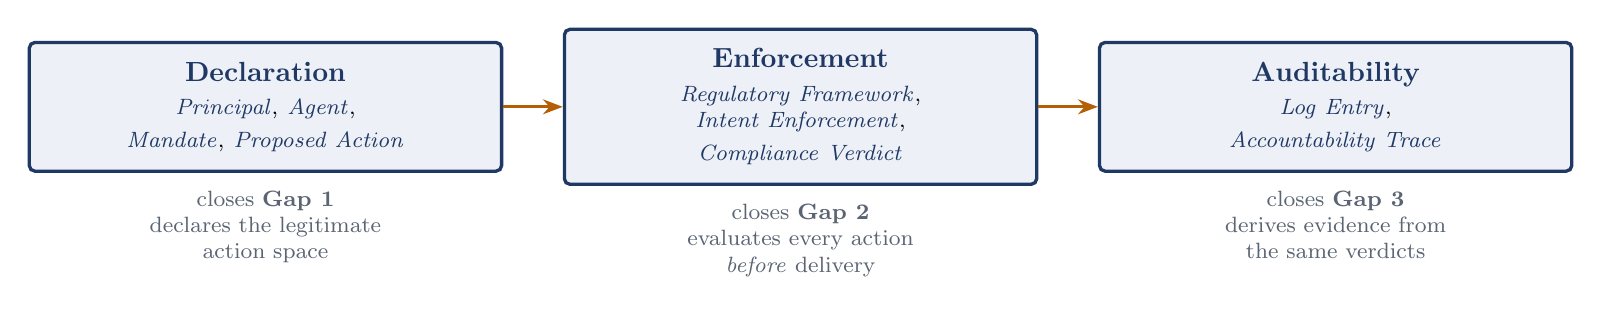
\begin{tikzpicture}[
      pil/.style={draw=aiPrimary,very thick,rounded corners=2pt,fill=aiLight,
                  text width=0.255\paperwidth,align=center,inner sep=7pt},
      lbl/.style={font=\footnotesize\color{aiGray},align=center},
      >={Stealth[length=2.5mm]}]
    \node[pil] (d) {\textbf{\color{aiPrimary}Declaration}\\[0.25em]
      {\footnotesize \cn{Principal}, \cn{Agent},\\ \cn{Mandate}, \cn{Proposed Action}}};
    \node[pil,right=0.035\paperwidth of d] (e) {\textbf{\color{aiPrimary}Enforcement}\\[0.25em]
      {\footnotesize \cn{Regulatory Framework},\\ \cn{Intent Enforcement},\\ \cn{Compliance Verdict}}};
    \node[pil,right=0.035\paperwidth of e] (a) {\textbf{\color{aiPrimary}Auditability}\\[0.25em]
      {\footnotesize \cn{Log Entry},\\ \cn{Accountability Trace}}};
    \draw[->,very thick,aiAccent] (d) -- (e);
    \draw[->,very thick,aiAccent] (e) -- (a);
    \node[lbl,below=3pt of d] {closes \textbf{Gap 1}\\ declares the legitimate\\ action space};
    \node[lbl,below=3pt of e] {closes \textbf{Gap 2}\\ evaluates every action\\ \emph{before} delivery};
    \node[lbl,below=3pt of a] {closes \textbf{Gap 3}\\ derives evidence from\\ the same verdicts};
  \end{tikzpicture}
  \end{center}
  \vspace{0.6em}
  \begin{block}{What \ai{} is --- and is not}
    \small
    \ai{} is \key{not} a new modeling language, nor a syntactic extension of one.
    It is a domain-independent \key{conceptual model}: governance constructs,
    their metamodel relationships, and well-formedness conditions --- grounded in
    \key{UFO}, rendered in OntoUML, and intended to \emph{augment} existing
    agent-oriented languages.
  \end{block}
\end{frame}

\begin{frame}{The conceptual model}
  \begin{center}
    \includegraphics[width=0.94\textwidth,height=0.72\textheight,keepaspectratio]%
      {pics/AI-Intent-Conceptual-Model_Enlarged.png}
  \end{center}
\end{frame}

\begin{frame}{Pillar 1 --- Declaration}{The Mandate is the central artifact}
  A \cn{Mandate} is a \key{type-level specification} of what an agent may
  address, what it must not produce, and its operational parameters:
  \medskip
  \begin{columns}[T,onlytextwidth]
    \begin{column}{0.48\textwidth}
      \begin{itemize}
        \item[(i)]   \cn{Decision Rights} --- decisions allowed without escalation
        \item[(ii)]  \cn{Boundaries} --- the negative obligations
        \item[(iii)] \cn{Capabilities} --- permitted tools, data, actuators
        \item[(iv)]  \cn{Policies} --- thresholds, escalation, revocation
      \end{itemize}
    \end{column}
    \begin{column}{0.48\textwidth}
      \begin{block}{Each boundary constraint is a triple}
        \[ c_i \;=\; \langle\, \mathit{text}_i,\; \phi_i,\; \tau_i \,\rangle \]
        \footnotesize
        $\mathit{text}_i$ --- natural-language statement\\
        $\phi_i$ --- machine-evaluable predicate over output\\
        $\tau_i \in \{\mathbf{F},\mathbf{O}\}$ --- prohibition or obligation
        \medskip

        A prohibition is violated \emph{iff} the output \emph{satisfies} $\phi_i$.
        A \key{risk parameter} binds a free variable in $\phi_i$:
        $\mathbf{F}(\mathit{allocation} > 0.15)$.
      \end{block}
    \end{column}
  \end{columns}
  \vspace{0.5em}
  \small A \cn{Proposed Action} is the candidate output \emph{before} evaluation ---
  the unit intercepted in Pillar 2.
\end{frame}

\begin{frame}{Pillar 2 --- Enforcement}{Defined by requirements, not by an algorithm}
  \cn{Intent Enforcement}, realized at runtime as a \key{Compliance Agent}, is the
  structural gatekeeper. As a framework construct it is defined by four
  \key{constitutive requirements}:
  \medskip
  \begin{columns}[T,onlytextwidth]
    \begin{column}{0.48\textwidth}
      \begin{block}{R1 --- Non-bypassability}
        \small Every cross-agent \cn{Proposed Action} is mediated. There is no
        delivery path that circumvents evaluation.
      \end{block}
      \begin{block}{R2 --- Independence}
        \small The evaluator is distinct from the agent evaluated, so enforcement
        does not inherit the generator's stochasticity.
      \end{block}
    \end{column}
    \begin{column}{0.48\textwidth}
      \begin{block}{R3 --- Verdict decidability}
        \small A determinate approve/block per constraint, naming the violated
        constraint when blocked.
      \end{block}
      \begin{block}{R4 --- Terminating revision}
        \small A bounded revision loop ending in delivery or a \key{recorded
        forced block} --- never in an unrecorded pass.
      \end{block}
    \end{column}
  \end{columns}
  \vspace{0.6em}
  \begin{center}\small
    \emph{How} a deployment discharges R1--R4 --- deterministic predicates,
    semantic classifier, hybrid --- is an implementation concern.
  \end{center}
\end{frame}

\begin{frame}{From risk parameter to verdict}{Worked example}
  \begin{center}
  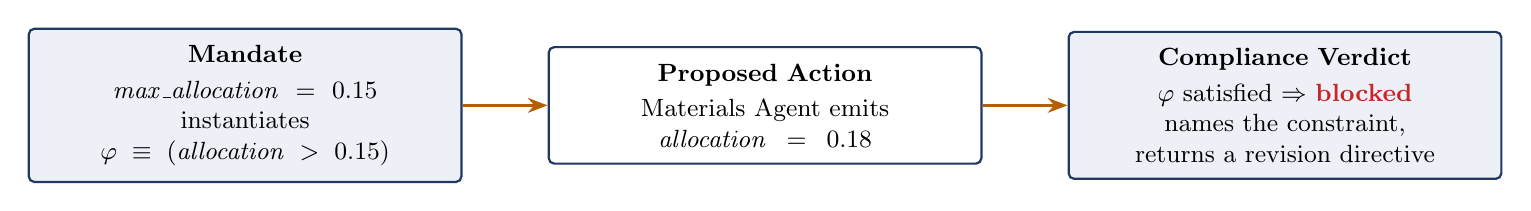
\begin{tikzpicture}[node distance=0.9em,>={Stealth[length=2.5mm]},
      bx/.style={draw=aiPrimary,thick,rounded corners=2pt,inner sep=6pt,
                 text width=0.235\paperwidth,align=center,font=\small}]
    \node[bx,fill=aiLight] (m) {\textbf{Mandate}\\[0.2em]
       $\mathit{max\_allocation}=0.15$\\ instantiates\\ $\varphi \equiv (\mathit{allocation} > 0.15)$};
    \node[bx,right=0.05\paperwidth of m,fill=white] (p) {\textbf{Proposed Action}\\[0.2em]
       Materials Agent emits\\ $\mathit{allocation}=0.18$};
    \node[bx,right=0.05\paperwidth of p,fill=aiLight] (v) {\textbf{Compliance Verdict}\\[0.2em]
       $\varphi$ satisfied $\Rightarrow$ \bad{\textbf{blocked}}\\
       names the constraint,\\ returns a revision directive};
    \draw[->,very thick,aiAccent] (m) -- (p);
    \draw[->,very thick,aiAccent] (p) -- (v);
  \end{tikzpicture}
  \end{center}
  \vspace{0.8em}
  \begin{block}{Why this matters for the model}
    The risk parameter supplies the \key{threshold}; the deontic type
    $\mathbf{F}$ supplies the \key{polarity}. Together they make the boundary
    predicate \key{decidable at runtime} --- risk parameters are not
    free-standing numbers but the operands of enforcement.
  \end{block}
\end{frame}

\begin{frame}{Pillar 3 --- Auditability}{Evidence, not logging}
  The \cn{Accountability Trace} is a UFO \emph{situation} aggregating the
  \cn{Log Entries} of a complete session:
  \[
    T(s) \;=\; \langle l_1,\dots,l_n \rangle
    \quad\text{closed under each } l_i\text{'s references to its Proposed Action and Mandate}
  \]
  \begin{columns}[T,onlytextwidth]
    \begin{column}{0.48\textwidth}
      \begin{block}{Two well-formedness conditions}
        \small
        \textbf{WFC-1} Every \cn{Compliance Verdict} is recorded in exactly one
        \cn{Log Entry} --- no evaluation is unlogged.\\[0.4em]
        \textbf{WFC-2} A completed session's Trace has a \cn{Log Entry} for every
        cross-agent \cn{Proposed Action} --- no action unaccounted for.
      \end{block}
    \end{column}
    \begin{column}{0.48\textwidth}
      \begin{block}{Why this is structural}
        \small
        A conventional audit log may be absent, partial or post-hoc-editable
        without violating any model constraint.\\[0.4em]
        Here a session missing a \cn{Log Entry} is \key{ill-formed by definition}
        --- and because the Trace derives from the \emph{same} verdicts that gate
        delivery, the record \key{cannot diverge} from what was enforced.
      \end{block}
    \end{column}
  \end{columns}
  \vspace{0.4em}
  \begin{center}\small
    Auditability is a \emph{consequence} of the enforcement structure,
    not a component bolted alongside it.
  \end{center}
\end{frame}

\begin{frame}{Ontological grounding in UFO}{\emph{der} = UFO-derived (inherits formal entailments) \quad \emph{des} = design choice layered on top}
  \centering\small
  \begin{tabularx}{0.97\textwidth}{@{}llXc@{}}
    \toprule
    \textbf{Pillar} & \textbf{Construct} & \textbf{UFO category, OntoUML stereotype} & \textbf{Src}\\
    \midrule
    \multirow{4}{*}{Declaration}
      & Principal            & Intentional object, \uml{kind}                                & des \\
      & Agent                & Intentional object w/ dispositions, \uml{kind}                & \textbf{der} \\
      & Mandate              & Normative description, \uml{description}                      & des \\
      & Proposed Action      & Event (non-repeatable), \uml{event}                           & \textbf{der} \\
    \midrule
    \multirow{3}{*}{Enforcement}
      & Regulatory Framework & External normative description, \uml{description}             & des \\
      & Intent Enforcement   & Role played by the (Compliance) Agent, \uml{role}             & des \\
      & Compliance Verdict   & Relator mediating enforcement and action, \uml{relator}       & des \\
    \midrule
    \multirow{2}{*}{Auditability}
      & Log Entry            & Persistent record of a compliance event, \uml{kind}           & des \\
      & Accountability Trace & Situation aggregating a session's Log Entries, \uml{situation}& \textbf{der} \\
    \bottomrule
  \end{tabularx}
  \vspace{0.7em}

  \small UFO is used for \key{ontological categorization} and its entailments ---
  \key{no UFO reasoner is required at runtime}.
\end{frame}

% =====================================================================
\section{Evaluation}

\begin{frame}{Reference implementation}{Private investment advisory under MiFID~II}
  \begin{columns}[T,onlytextwidth]
    \begin{column}{0.52\textwidth}
      \begin{center}
      \resizebox{\linewidth}{!}{%
      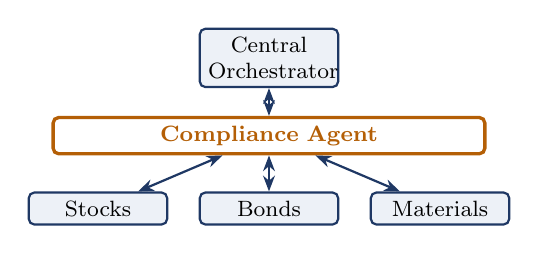
\begin{tikzpicture}[>={Stealth[length=2mm]},font=\footnotesize,
        ag/.style={draw=aiPrimary,thick,rounded corners=2pt,fill=aiLight,
                   inner sep=3pt,text width=4.4em,align=center},
        gate/.style={draw=aiAccent,very thick,rounded corners=2pt,fill=white,
                   inner sep=3pt,text width=15em,align=center}]
        \node[ag] (c) {Central\\Orchestrator};
        \node[gate,below=1.0em of c] (g) {\textbf{\color{aiAccent}Compliance Agent}};
        \node[ag,below=1.3em of g] (b) {Bonds};
        \node[ag,left=1.1em of b] (s) {Stocks};
        \node[ag,right=1.1em of b] (m) {Materials};
        \draw[<->,thick,aiPrimary] (c) -- (g);
        \draw[<->,thick,aiPrimary] (g) -- (s);
        \draw[<->,thick,aiPrimary] (g) -- (b);
        \draw[<->,thick,aiPrimary] (g) -- (m);
      \end{tikzpicture}}
      \end{center}
      \vspace{-0.3em}
      {\footnotesize\color{aiGray}\centering
       No sub-agent is reachable except through the Compliance Agent --- R1.\par}
    \end{column}
    \begin{column}{0.45\textwidth}
      \footnotesize
      \begin{tabular}{@{}lccl@{}}
        \toprule
        \textbf{Agent} & $|C|$ & $|R|$ & \textbf{Example constraint} \\
        \midrule
        Central   & 5 & 2 & $\mathbf{F}$(class $>40\%$) \\
        Stocks    & 5 & 3 & $\mathbf{F}$(position $>10\%$) \\
        Bonds     & 5 & 4 & $\mathbf{F}$(duration $>10$\,yr) \\
        Materials & 5 & 4 & $\mathbf{F}$(allocation $>15\%$) \\
        \bottomrule
      \end{tabular}
      \vspace{0.8em}

      \footnotesize
      \key{Why this domain?} MiFID~II supplies \emph{externally given}
      constraints --- imposed by regulation, not authored by us.
      \medskip

      \key{Stack:} Python 3.11+, Pydantic v2, SQLite, Streamlit,
      Llama~3.1~8B served locally via Ollama.
    \end{column}
  \end{columns}
\end{frame}

\begin{frame}{The constructs, made operable}{Dashboard of the reference implementation}
  \begin{center}
    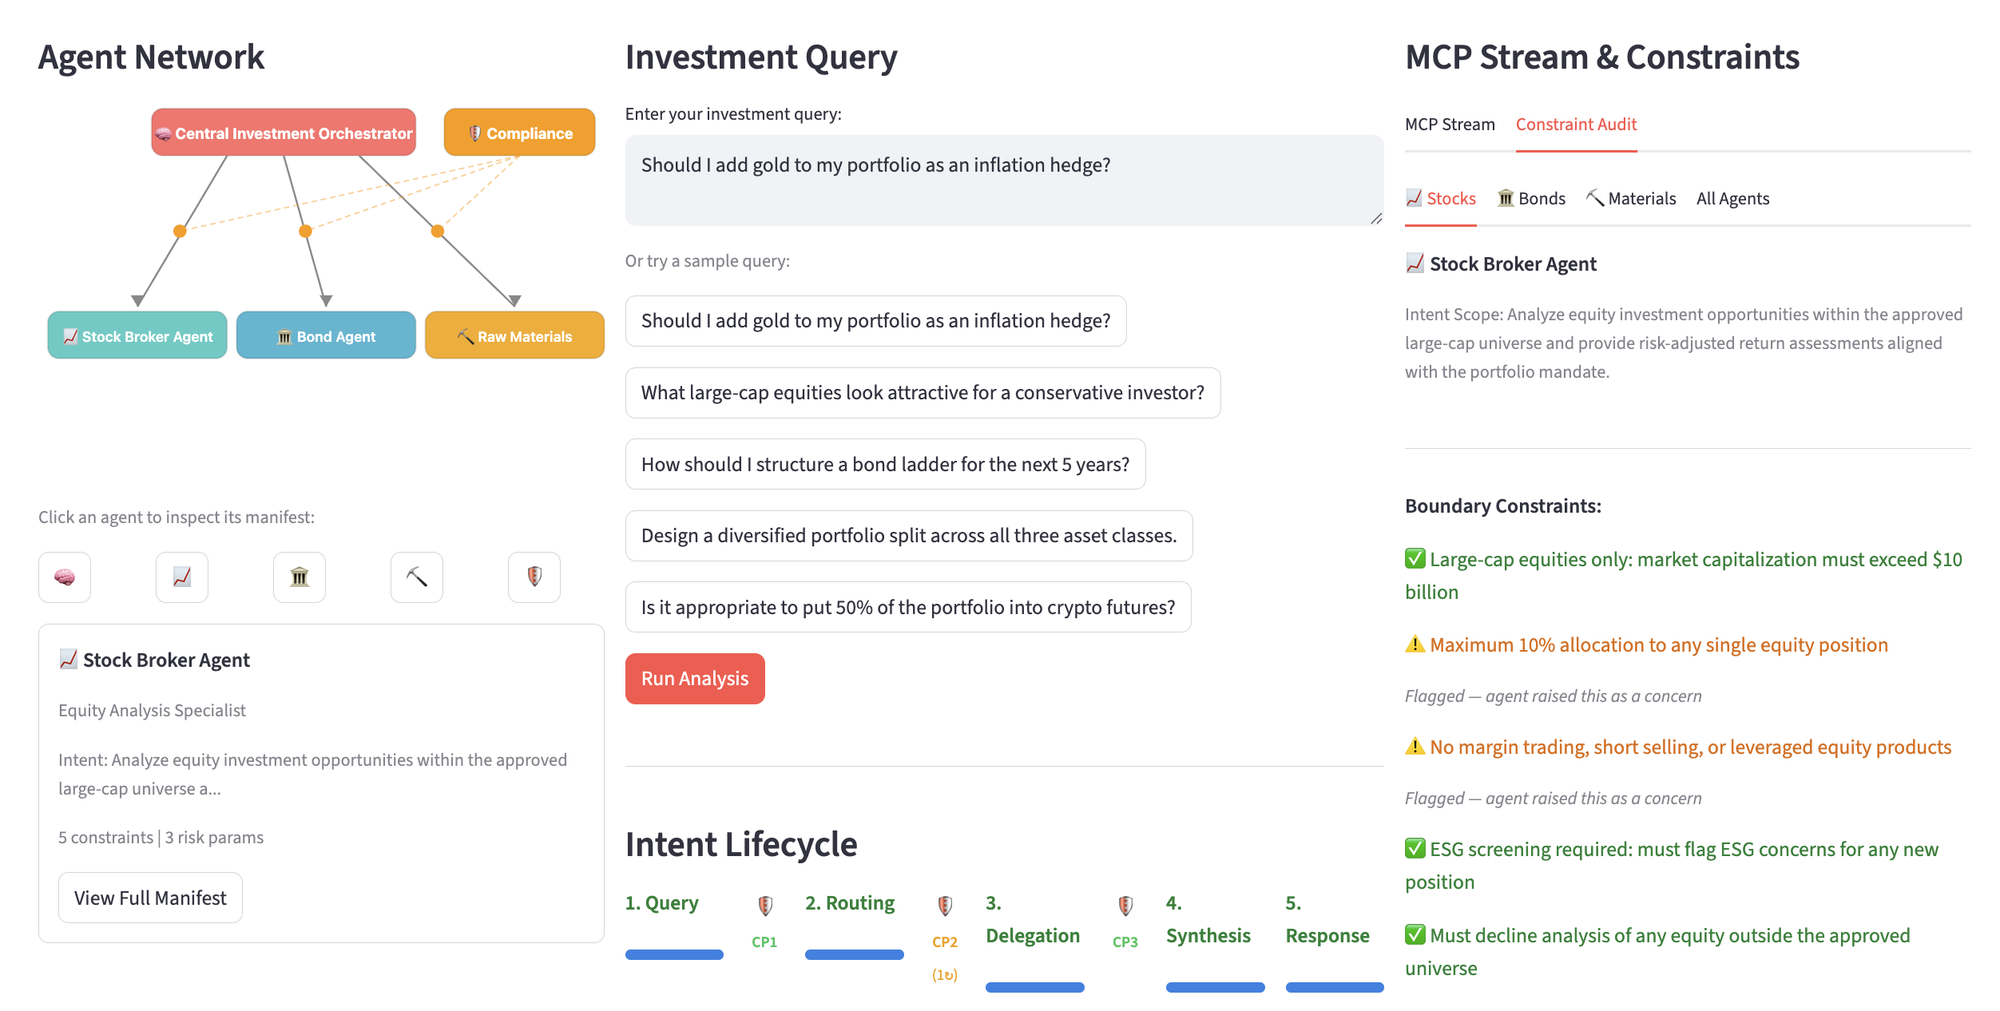
\includegraphics[width=\textwidth,height=0.615\textheight,keepaspectratio]{pics/app-dashboard-wide.png}
  \end{center}
  \vspace{-0.2em}
  \begin{columns}[T,onlytextwidth]
    \begin{column}{0.31\textwidth}
      \scriptsize\textbf{\color{aiPrimary}Agent Network}\\
      The \cn{Compliance Agent} sits on every Orchestrator--sub-agent edge ---
      \key{R1}.
    \end{column}
    \begin{column}{0.33\textwidth}
      \scriptsize\textbf{\color{aiPrimary}Intent Lifecycle}\\
      Query $\to$ Routing $\to$ Delegation $\to$ Synthesis $\to$ Response,
      with a \key{checkpoint} between stages.
    \end{column}
    \begin{column}{0.33\textwidth}
      \scriptsize\textbf{\color{aiPrimary}Constraint Audit}\\
      Per-agent \cn{Mandate}: intent scope, each constraint with its status,
      the \cn{risk parameters}.
    \end{column}
  \end{columns}
\end{frame}

\begin{frame}{What the gate actually produces}{Constraint Audit for the Stocks Agent, one session}
  \begin{columns}[c,onlytextwidth]
    \begin{column}{0.44\textwidth}
      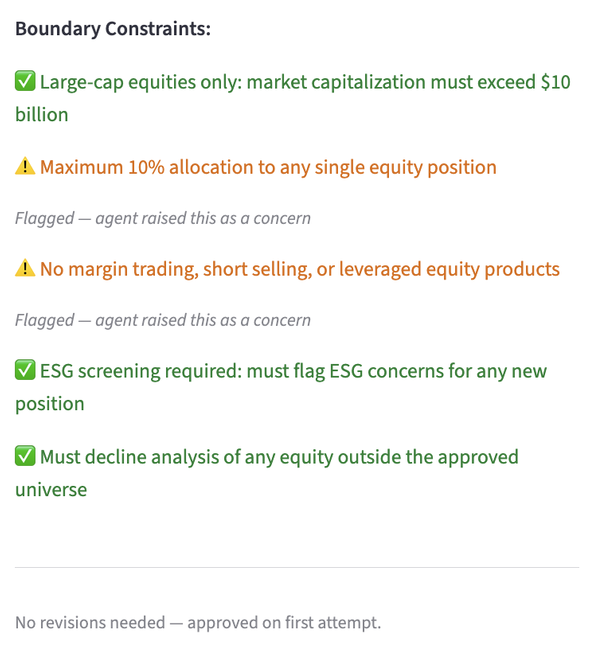
\includegraphics[width=\linewidth]{pics/app-audit.png}
    \end{column}
    \begin{column}{0.52\textwidth}
      \small
      All five boundary constraints of the Stocks \cn{Mandate} are evaluated and
      reported \key{individually} --- \ok{satisfied} or
      \textcolor{aiAccent}{flagged by the agent as a concern}.
      \medskip

      This is the \cn{Compliance Verdict} made visible: not a pass/fail score,
      but a per-constraint record naming what was checked.
      \medskip

      That record is exactly what \cn{Log Entries} carry, and what the
      \cn{Accountability Trace} aggregates --- \key{WFC-1} and \key{WFC-2}
      are satisfied by construction, not by a reporting step.
      \medskip

      {\color{aiGray}Here the Stocks agent was approved on its first attempt.
       The session's one revision happened elsewhere --- next slide.}
    \end{column}
  \end{columns}
\end{frame}

\begin{frame}{Communication as evidence}{The same session, as the MCP message log}
  \begin{columns}[c,onlytextwidth]
    \begin{column}{0.50\textwidth}
      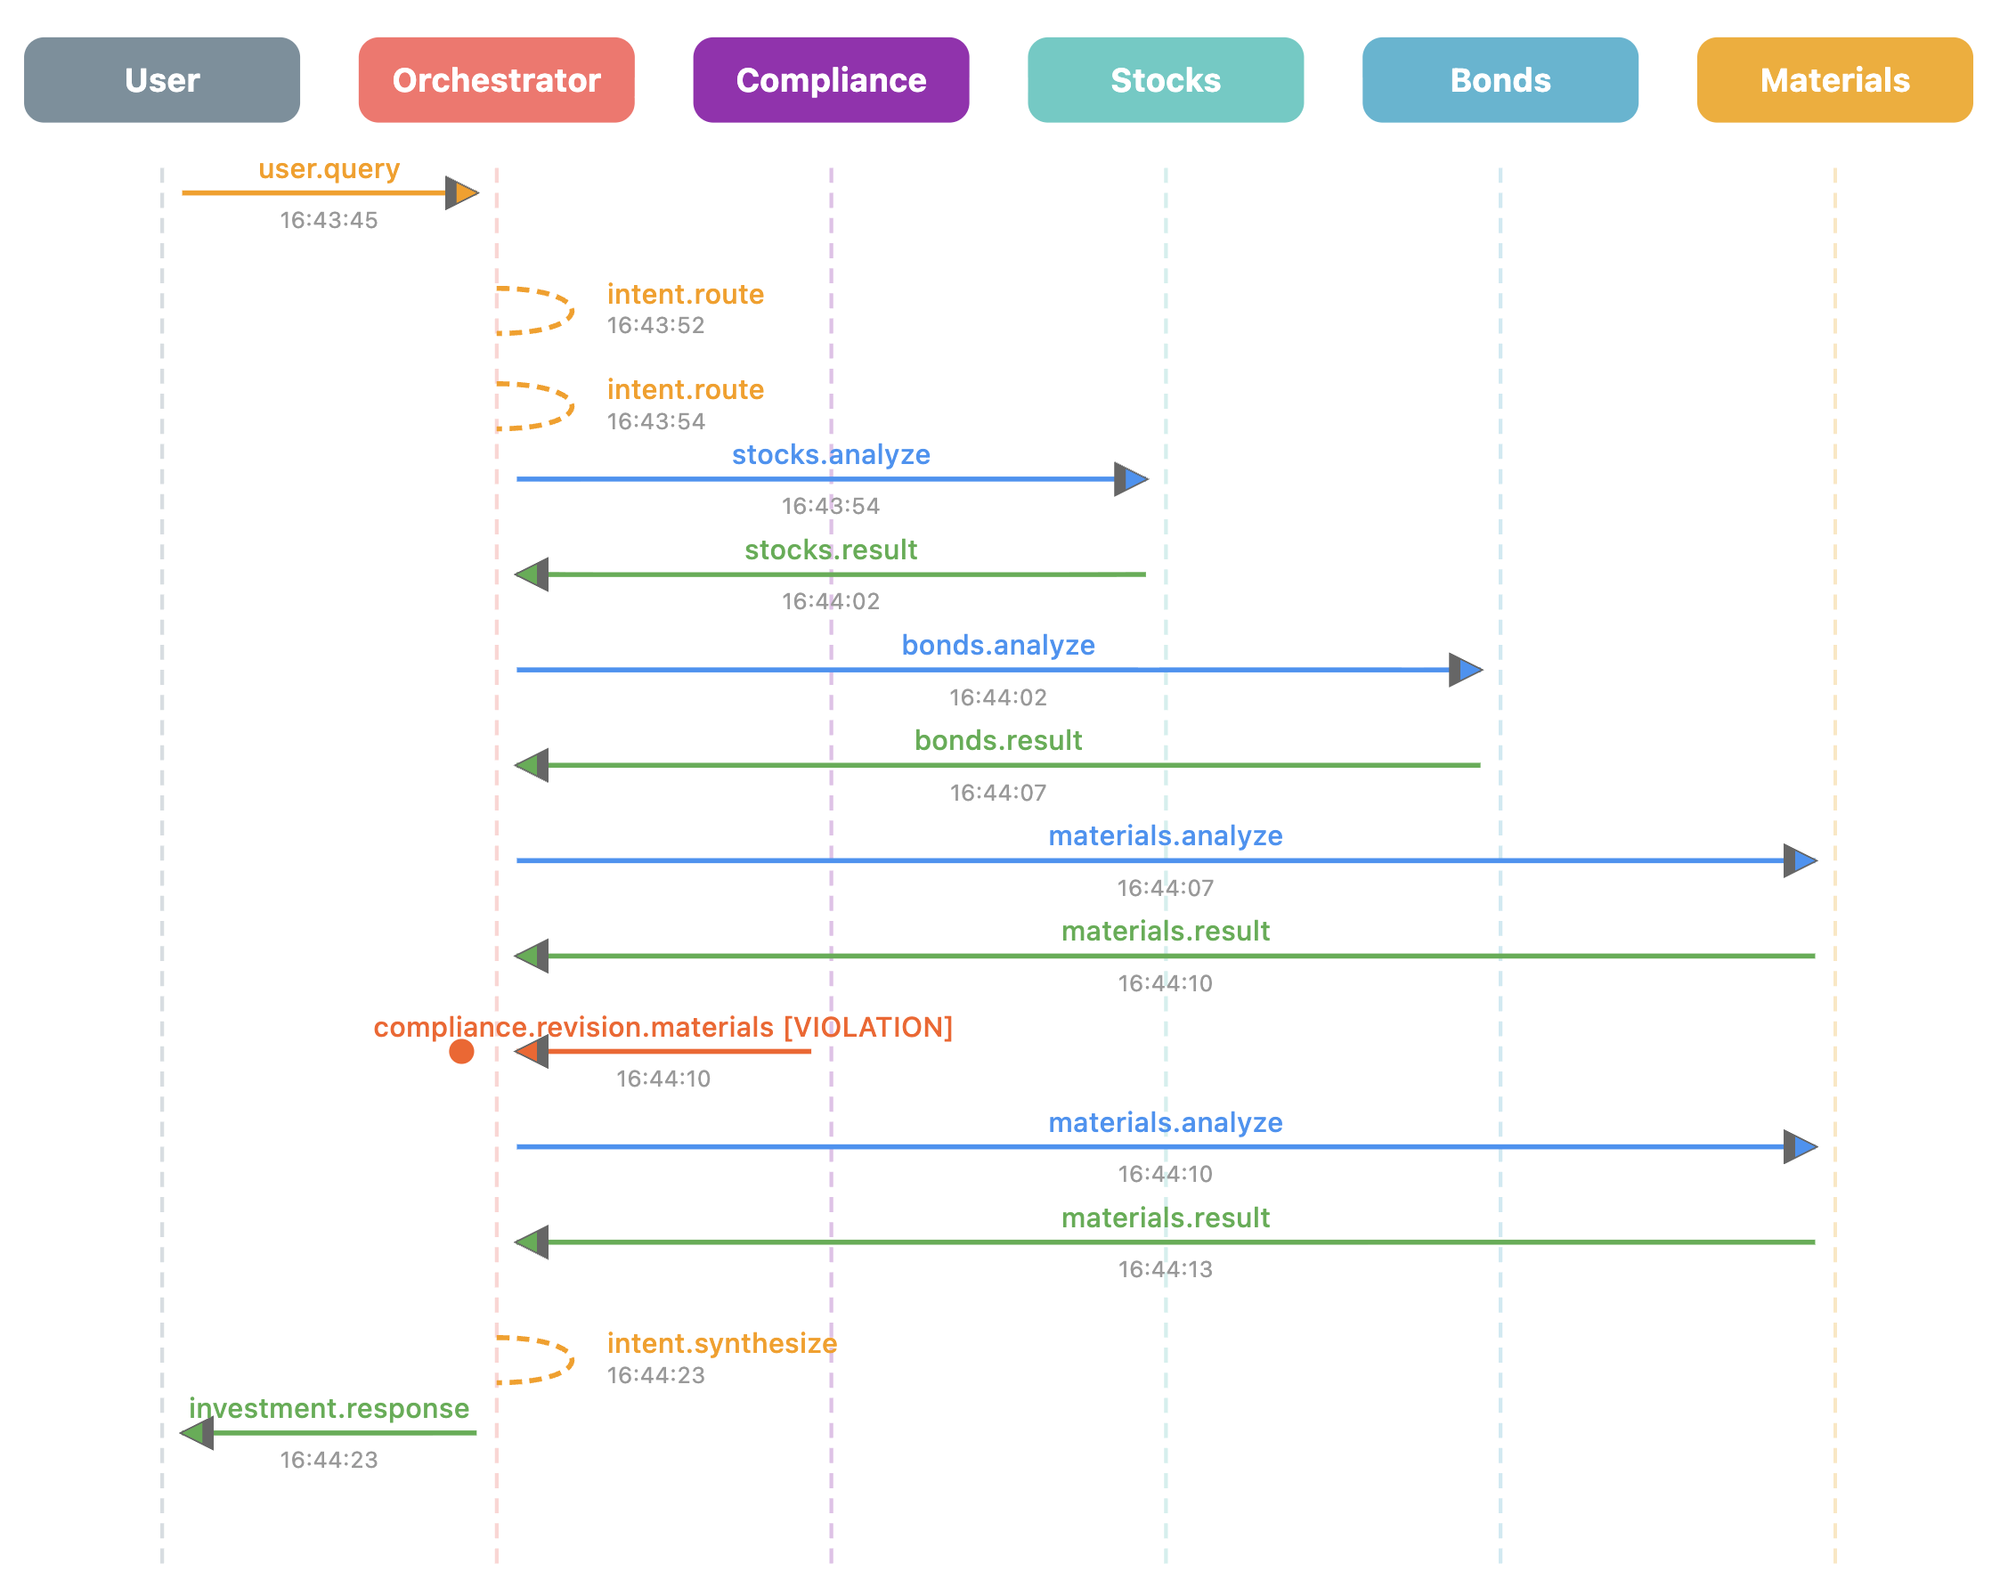
\includegraphics[width=\linewidth,height=0.86\textheight,keepaspectratio]{pics/app-mcp-sequence.png}
    \end{column}
    \begin{column}{0.465\textwidth}
      \small
      Every inter-agent action is a \key{time-indexed, non-repeatable event} ---
      the UFO categorization that licenses its use as evidence.
      \medskip

      The whole session is reconstructible from this log alone: routing, each
      delegation and result, the compliance event, the synthesis, and the
      response to the user.
      \medskip

      \textbf{\color{aiWarn}\texttt{compliance.revision.materials [VIOLATION]}}
      at 16:44:10 is the gate firing --- and it is \emph{in the record},
      not inferred from it.
      \medskip

      {\color{aiGray}This is scenario \textbf{S3}, audit reconstruction: no
       existing agent-oriented framework provides an equivalent artifact as a
       structural model component.}
    \end{column}
  \end{columns}
\end{frame}

\begin{frame}{The revision loop, R4, in one session}
  \begin{center}
    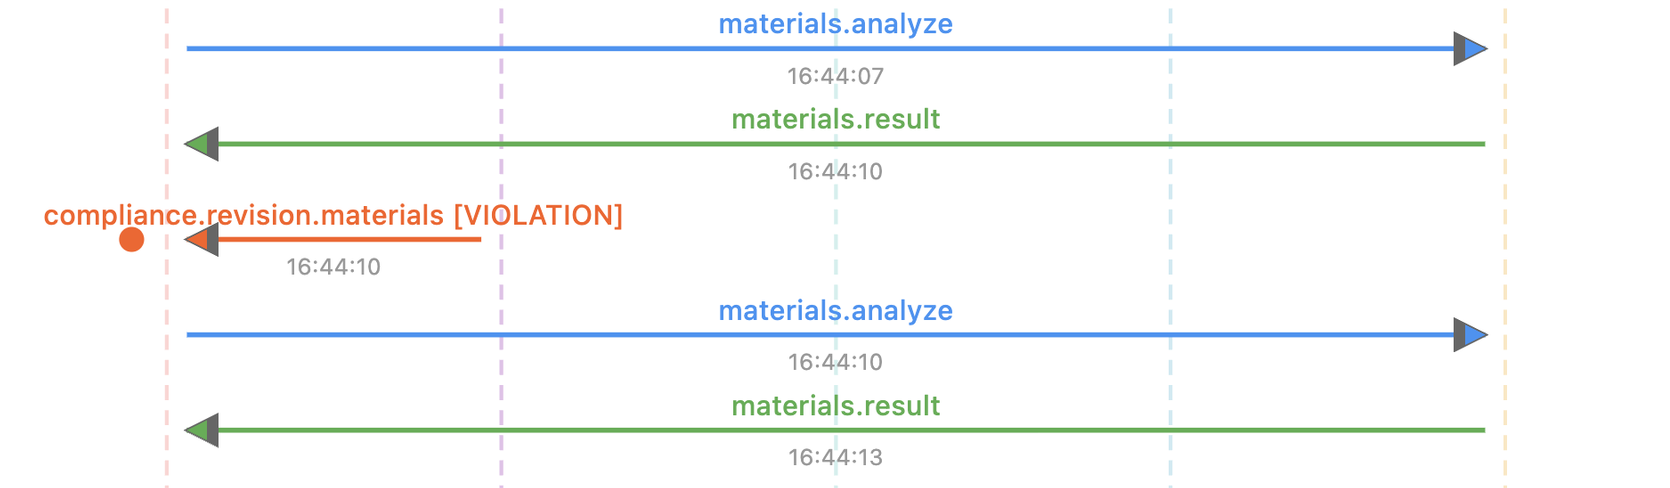
\includegraphics[width=\textwidth]{pics/app-revision-loop.png}
  \end{center}
  \vspace{0.3em}
  \begin{columns}[T,onlytextwidth]
    \begin{column}{0.48\textwidth}
      \footnotesize
      The Materials Agent answers at \texttt{16:44:10}. The Compliance Agent
      evaluates the \cn{Proposed Action} against the Materials \cn{Mandate},
      finds a violated boundary constraint, and returns a
      \key{revision directive} instead of delivering.
    \end{column}
    \begin{column}{0.48\textwidth}
      \footnotesize
      The agent re-analyses and answers again at \texttt{16:44:13}; that
      response is delivered. \key{One revision, zero forced blocks} --- a
      bounded loop terminating in delivery, exactly what \key{R4} requires.
      \emph{The non-compliant first answer never reached the Orchestrator.}
    \end{column}
  \end{columns}
\end{frame}

\begin{frame}{Two claims, two evaluations}
  \begin{columns}[T,onlytextwidth]
    \begin{column}{0.48\textwidth}
      \begin{block}{Expressiveness --- the \emph{modeling} claim}
        \footnotesize
        Scenarios S1--S3 instantiate the three gaps and exercise the three
        pillars. Does each capture a scenario existing agent-oriented
        languages do not?
      \end{block}
      \footnotesize
      \textbf{S1 Out-of-scope declination.} Agents returned
      \texttt{out\_of\_scope:true} with named constraints (stocks asked about
      gold). \emph{GAIA can express the permission but not verify it;
      $i^*$ has no prohibition construct.}
      \medskip

      \textbf{S2 Quantitative enforcement.} The checker fired on every session
      exceeding a quantitative limit. \emph{NMAS needs the agent to evaluate
      itself; GAIA has no quantitative construct.}
      \medskip

      \textbf{S3 Audit reconstruction.} Full decision sequence reconstructible
      from the Trace. \emph{No existing framework offers an equivalent artifact.}
    \end{column}
    \begin{column}{0.48\textwidth}
      \begin{block}{Applicability --- the \emph{operativity} claim}
        \footnotesize
        Do the constructs hold at runtime, across sessions and \emph{adversarial
        agent dispositions}?
      \end{block}
      \footnotesize
      \textbf{19 test cases}
      \begin{itemize}\footnotesize
        \item TC-1--15: in-scope baseline, out-of-scope, hard constraint
              violation, synthesis and trace integrity
        \item TC-16--19: disposition presets --- \emph{Neutral}, \emph{Aggressive
              Broker}, \emph{Reckless Portfolio Manager}, \emph{Groupthink}
      \end{itemize}
      \medskip
      \textbf{10 independent runs $\Rightarrow$ 190 evaluations}
      \medskip

      Scoring is \key{deterministic pattern matching} over session JSON
      (allocation regexes, rule-ID lookup, field presence) --- 0, 1 or 2 per
      dimension. \key{No LLM judge.}
    \end{column}
  \end{columns}
\end{frame}

\begin{frame}{Results across 190 evaluations}
  \centering\small
  \begin{tabularx}{0.97\textwidth}{@{}lXccll@{}}
    \toprule
    \textbf{Dim.} & \textbf{Framework claim} & \textbf{Thr.} & \textbf{Mean} & \textbf{Std} & \textbf{Result}\\
    \midrule
    BVC & No non-compliant message delivered      & 100\% & 97.9\% & 2.7  & Near-pass \\
    CGP & No compliant response falsely blocked   & 85\%  & 97.9\% & 2.7  & \ok{Pass} \\
    ATC & Traces carry session, agent, rule IDs   & 80\%  & 71.3\% & 5.3  & \bad{Below} \\
    CDA & Violations caught on first evaluation   & 90\%  & 38.6$_u$/50.6$_c$\% & 5.3 & \bad{Below} \\
    ME  & Out-of-scope declined with constraint name & 75\% & 35.0\% & 22.9 & Volatile \\
    DC  & Output within limits under any preset   & ---   & 57.5$_s$\% & 36.8 & Strict \\
    \bottomrule
  \end{tabularx}
  \vspace{0.5em}

  {\footnotesize\color{aiGray}
   BVC Boundary Violation Containment $\cdot$ CGP Compliance Gate Precision $\cdot$
   ATC Accountability Trace Completeness\\
   CDA Constraint Detection Accuracy ($u$ unconditioned, $c$ conditioned) $\cdot$
   ME Mandate Enforcement $\cdot$ DC Disposition Containment ($s$ strict)}
  \vspace{0.9em}

  \begin{block}{The headline}
    \key{Zero forced-pass across all 190 evaluations.} Every violation that
    occurred was eventually caught before delivery.
  \end{block}
\end{frame}

\begin{frame}{Reading the numbers honestly}
  \small
  \begin{columns}[T,onlytextwidth]
    \begin{column}{0.48\textwidth}
      \textbf{BVC / CGP (both 97.9\%)} co-occur exactly --- they measure the same
      event. In 6 of 10 runs nothing non-compliant was delivered. The other four
      each involved \emph{one} borderline case: 14.8\% gold under
      \emph{reckless\_portfolio} --- within the 15\% limit, correctly approved by
      the numerical criterion, but the phrasing implied intended circumvention
      the predicate does not capture.
      \medskip

      \textbf{ATC (71.3\%)} Traces were structurally well-formed in
      \emph{every} session. Llama~3.1~8B omitted violated rule identifiers in
      28.7\%. An \key{instruction-following limit of a small model}, not a
      design failure.
    \end{column}
    \begin{column}{0.48\textwidth}
      \textbf{CDA (50.6\% conditioned)} measures detection \key{latency}, not
      reliability: violations caught on revision 2 or later rather than first.
      Every violation was still caught before delivery --- sufficient for
      containment in a revision-based architecture.
      \medskip

      \textbf{ME (35.0\%, std 22.9)} reflects \key{routing non-determinism}, not
      enforcement failure: when the orchestrator did not route to the target
      agent, the mandate could not be tested. An evaluation-methodology finding.
      \medskip

      \textbf{DC (57.5\% strict)} No forced-pass in 40 disposition evaluations.
      \emph{reckless\_portfolio} triggered 2--5$\times$ more revisions but
      \key{never breached the gate}. A measure of compliance \emph{effort}, not safety.
    \end{column}
  \end{columns}
\end{frame}

% =====================================================================
\section{Discussion}

\begin{frame}{What AI-Intent contributes --- and what it costs}
  \begin{block}{Three modeling constructs existing frameworks lack}
    \small
    \textbf{1. Binary sortal boundary} on the action space --- complementary to
    graded goals, made explicit as a first-class enforceable artifact.\\[0.3em]
    \textbf{2. External norm enforcement} as a structural role rather than agent
    self-compliance --- motivated by first-attempt violation rates observed
    \emph{even under a neutral disposition}: \key{12.9\%} for the materials
    agent, \key{25.6\%} overall.\\[0.3em]
    \textbf{3. Communication-as-evidence} --- a \cn{Compliance Verdict} attached
    to every message, with the Trace derived from it.
  \end{block}
  \begin{block}{The compliance--utility tension}
    \small
    Asked for a leveraged gold ETF --- a product the Materials Mandate forbids ---
    the Materials Agent was permanently blocked and the Orchestrator fell back on
    Stocks and Bonds, producing a \emph{fully compliant recommendation that did
    not answer the question posed}.\\[0.3em]
    \ai{} resolves this by giving constraints \key{lexicographic priority}: a
    compliant non-answer beats a non-compliant answer. Right for regulated
    finance --- but currently \emph{implicit} rather than modeled.
  \end{block}
\end{frame}

\begin{frame}{Limitations we take seriously}
  \small
  \begin{itemize}
    \item \textbf{Modeling-scope boundaries.} Constraint conflicts are detected
      but not resolved; Mandates are immutable at runtime; constraints have
      \emph{no exception structure}, unlike defeasible deontic logic --- deliberate
      for regulated finance, limiting where exceptions are routine.
    \medskip
    \item \textbf{Specification--predicate consistency.} If $\phi_i$ is miscoded
      relative to $\mathit{text}_i$, the gate silently enforces the wrong rule.
      A cap coded as $>0.20$ where the text says 15\% yields a \key{silent false
      pass} --- and \key{BVC still reports containment, because no rule fired}.
      The metric cannot detect its own predicate being wrong. Our expected rules
      and enforced predicates \emph{share provenance}, so the evaluation does not
      independently verify this.
    \medskip
    \item \textbf{Model operativity depends on instruction following.}
      Model-agnostic by design, model-dependent in practice.
    \medskip
    \item \textbf{Deterministic predicate checking.} Substring matching for
      leverage detection fires on false positives; a 15-word negation window
      suppresses ``not''/``avoid''/``decline'', but not every formulation.
    \medskip
    \item \textbf{Routing non-determinism} leaves mandate enforcement untestable
      when the target agent is never invoked.
  \end{itemize}
\end{frame}

\begin{frame}{Conclusion}
  \begin{block}{The argument}
    \small
    \ai{} grounds three governance constructs --- a \key{binary action-space
    boundary}, \key{runtime-enforceable negative obligations}, and
    \key{communication-as-evidence} --- in deontic logic and UFO, distinguishing
    what is \emph{new} (sortal boundaries, external norm enforcement) from what is
    \emph{appropriated} (prohibition semantics from NMAS, event ontology from UFO).
  \end{block}
  \begin{block}{What the reference implementation supports}
    \small
    (i) Agent self-compliance is unreliable for non-deterministic generators ---
    motivating external enforcement as a \emph{structural}, not optional, component.\\[0.3em]
    (ii) A Compliance Agent realizing R1--R4 can contain boundary violations
    \emph{even under adversarial agent dispositions}.
  \end{block}
  \begin{block}{Future work --- three tracks}
    \small
    \textbf{Modeling:} defeasible norms, session-mutable Mandates, richer predicates.
    \quad\textbf{Ontological:} a full OntoUML model, and whether design-time
    reasoning catches the specification--predicate inconsistencies the runtime gate
    cannot. \quad\textbf{Empirical:} further domains, more capable models.
  \end{block}
\end{frame}

\begin{frame}[plain,noframenumbering]
  \vfill
  \begin{center}
    {\color{aiAccent}\rule{2.2em}{2.5pt}}\\[0.8em]
    {\LARGE\bfseries\color{aiPrimary}Thank you}\\[1.2em]
    {\large\color{aiPrimary}Questions?}\\[1.6em]
    {\footnotesize\color{aiGray}
      Wolfgang Maass \quad\texttt{wolfgang.maass@dfki.de}\\
      Iris Reinhartz-Berger \quad\texttt{iris@is.haifa.ac.il}\\[0.8em]
      Reference implementation, evaluation suite and data:\\
      \texttt{github.com/InformationServiceSystems/ai-intent}}
  \end{center}
  \vfill
\end{frame}

% =====================================================================
\appendix

\begin{frame}{Backup --- Agent mandates in full}
  \centering\footnotesize
  \begin{tabularx}{0.97\textwidth}{@{}p{1.7cm} p{2.3cm} cc X@{}}
    \toprule
    \textbf{Agent} & \textbf{Role} & $|C|$ & $|R|$ & \textbf{Key constraints (examples)}\\
    \midrule
    Central & Orchestrator & 5 & 2 &
      $\mathbf{F}$(single asset class $>40\%$); $\mathbf{O}$(consult $\geq1$ sub-agent);
      $\mathbf{O}$(surface all violations)\\
    \midrule
    Stocks & Equity Analyst & 5 & 3 &
      $\mathbf{F}$(non-large-cap); $\mathbf{F}$(position $>10\%$);
      $\mathbf{F}$(leverage); $\mathbf{O}$(ESG screening)\\
    \midrule
    Bonds & Fixed Income & 5 & 4 &
      $\mathbf{F}$(rating $<\mathrm{BBB{+}}$); $\mathbf{F}$(duration $>10$\,yr);
      $\mathbf{F}$(EM debt); $\mathbf{F}$(bucket $>30\%$/yr)\\
    \midrule
    Materials & Commodities & 5 & 4 &
      $\mathbf{F}$(non-Au/Ag commodity); $\mathbf{F}$(allocation $>15\%$);
      $\mathbf{F}$(leveraged ETF/futures); $\mathbf{O}$(inflation rationale)\\
    \bottomrule
  \end{tabularx}
  \vspace{0.6em}

  {\footnotesize $|C|$ = boundary constraints \quad $|R|$ = risk parameters}
\end{frame}

\begin{frame}{Backup --- Threats to validity}
  \small
  \textbf{Internal.} Scoring is deterministic pattern matching over session JSON,
  eliminating evaluator subjectivity. Expected rules were derived directly from
  Mandate definitions to mitigate misspecification.
  \medskip

  \textbf{External.} One domain (investment advisory), one model
  (Llama~3.1~8B) --- positioned as a \key{proof of concept}. The
  domain-independent core (metamodel, pillars, well-formedness conditions) is
  separable from domain-specific content and should transfer where
  \begin{enumerate}\footnotesize
    \item competence admits a sortal in/out-of-scope boundary,
    \item norms are prohibitions expressible as machine-evaluable predicates,
    \item Mandates are session-stable, and
    \item the domain tolerates lexicographic constraint priority.
  \end{enumerate}
  Transfer is poor where norms admit routine exceptions, resist decidable
  predicates, or require dynamic renegotiation.
  \medskip

  \textbf{Construct.} ATC measures trace-\emph{population} completeness, not
  semantic correctness; CDA measures detection \emph{latency}, not reliability.
  \medskip

  \textbf{Conclusion.} BVC/CGP variance across 10 runs is 2.7\% --- low enough to
  support containment under these conditions. The sharper claim, that adversarial
  dispositions never breach the gate, is supported \emph{categorically} (zero
  forced-pass in 40 disposition evaluations) rather than statistically.
\end{frame}

\end{document}
